\scanpage{199}
\[\tau=\operatorname{Tr}(x_1x_2)x_3x_4\qquad x_2x_1\]
\figure{\begin{tikzpicture}[scale=.55]
\draw[very thick] (0,2.7)--(.8,3.4);\draw (.95,3.3)--(1.6,2.8);
\draw[very thick] (1.5,2.6)--(.8,1.95);\draw (0,2.7)--(.6,2.05);
\draw[->] (.5,2.05)..controls (-.1,2.8) and (-.25,2.6)..(.1,2.5);
\draw[->,thick] (.15,1.4)..controls (-1,.7) and (.1,-.8)..(.8,.1)..controls (1.2,.8) and (.95,1.3)..(.65,1.3);
\draw[brown,very thick] (6,2.7)--(7,2.8);\fill (7.5,2.8) circle(.025);\fill (8,2.9) circle(.025);
\end{tikzpicture}}
\[\tau^2-\Sigma_{(1,2),3,4}\tau+\Pi\]
\[\operatorname{Tr}x_1x_2x_3\unsure{x_4}
 +\operatorname{Tr}x_2x_1x_3x_4\]
\[
\begin{gathered}
x_1x_2x_3x_4\qquad x_2x_3x_4x_1\qquad x_3x_4x_1x_2\qquad x_4x_1x_2x_3\\
x_4x_3x_2x_1\qquad x_3x_2x_1\qquad\tau
\end{gathered}
\]
\figure{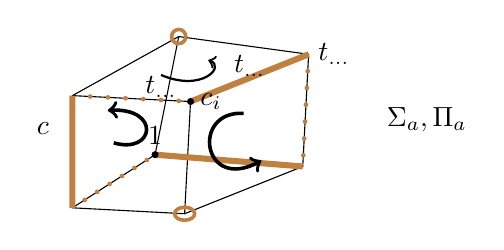
\begin{tikzpicture}[scale=.75]
\coordinate (a) at (0,2);\coordinate (b) at (2,1.9);
\coordinate (c) at (1.9,0);\coordinate (d) at (0,.1);
\coordinate (e) at (1.8,3);\coordinate (f) at (4,2.7);
\coordinate (g) at (3.9,.8);\coordinate (h) at (1.4,1);
\draw (a)--(b)--(c)--(d)--cycle;
\draw (e)--(f)--(g)--(h)--cycle;\draw (a)--(e) (b)--(f) (c)--(g) (d)--(h);
\draw[brown,line width=2.2pt] (a)--(d) (b)--(f) (h)--(g);
\foreach \u in {.15,.3,.45,.6,.75,.9}{
 \fill[brown] (\u*2,2-\u*.1) circle(.04);
 \fill[brown] (\u*1.4,.1+\u*.9) circle(.04);
 \fill[brown] (4-\u*.1,2.7-\u*1.9) circle(.04);}
\draw[brown,line width=1.3pt] (e) circle(.12);\draw[brown,line width=1.3pt] (c) ellipse(.17 and .11);
\fill (b) circle(.06);\fill (h) circle(.06);
\draw[->,thick] (1.5,2.35)..controls (2.2,2.05) and (2.6,2.5)..(2.3,2.6);
\draw[->,line width=1.3pt] (.7,1.2)..controls (1.4,1) and (1.5,1.8)..(.6,1.75);
\draw[->,line width=1.3pt] (2.9,1.7)..controls (2,1.75) and (2.2,.35)..(3.2,.9);
\node at (-.5,1.45) {$\unsure{c}$};\node[above] at (1.5,1.8) {$t_{\ldots}$};
\node[right] at (b) {$c_i$};\node[above] at (3,2.15) {$t_{\ldots}$};
\node[right] at (f) {$t_{\ldots}$};\node[above] at (h) {$1$};
\node at (6,1.6) {$\Sigma_a,\Pi_a$};
\end{tikzpicture}}
\[\deleted{\unsure{\tau}}\qquad\tau^2\]
\[\tau^{\unsure{8|\infty}}+\alpha_1\tau^7\;\text{---}\;+\alpha_8=0
\qquad\alpha_i\in\mathbb Z[b_{\cdot\cdot},c_\cdot,t_{\cdot\cdot}]\]
\[
\underbrace{b_s,c_s},t_s\ \big|\ \underbrace{t_a}\ \big|\ t_f
\]
\uline{Nb}
\[
\left\{\begin{aligned}b_s&=b_{s'}\\c_s&=c_{s'}\\t_a&=t_{a'}\end{aligned}\right.
\qquad\text{mais}\quad
\left\{\begin{aligned}
t_s&\ne t_{s'}&&\text{de degré }2\text{ sur }\unsure{A^{\mathfrak S_4}}\\
&&&\text{de degré }8\text{ sur }\unsure{A^{\mathfrak S_3}}\\
t_f&\ne t_{f'}&&\uline{\text{de degré }6\text{ sur }\unsure{B^{\mathfrak S_4}}}\\
&&&\text{de degré }8\ (?)\ \deleted{\unsure{4}}\text{ sur }A
\end{aligned}\right.
\]
\[
\begin{gathered}g\unsure{\tau|\bar\tau}\quad g'\tau\quad g''\tau\\
\sum g\tau\\\sum g\end{gathered}
\qquad
\begin{gathered}
\tau^{\unsure{8|\infty}}+\beta_1\tau^7\;\text{---}\;+\beta_8=0\\
\underbrace{(\alpha_1-\beta_1)}_{\gamma_1}\tau^7\;\text{---}\;+
 \underbrace{\alpha_8-\beta_8}=0
\end{gathered}
\]
\figure{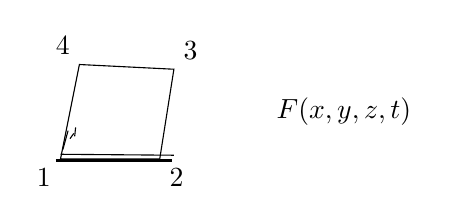
\begin{tikzpicture}[scale=.6]
\draw (0,0)--(.4,2)--(2.4,1.9)--(2.1,0)--cycle;
\draw[very thick] (-.1,-.03)--(2.35,-.03);\draw (0,.1)--(2.4,.08);
\draw (.05,.2)--(.16,.6);\draw (.2,.43)--(.28,.54);\draw (.3,.48)--(.32,.67);
\node[below left] at (0,0) {$1$};\node[below right] at (2.1,0) {$2$};
\node[above right] at (2.4,1.9) {$3$};\node[above left] at (.4,2) {$4$};
\node at (6,1) {$F(x,\uline{y,z},t)$};
\end{tikzpicture}}
\[H\subset\mathfrak S_4\]
\diagram{\begin{tikzcd}[ampersand replacement=\&]
B^H\arrow[d,dash,"\text{degré }6"]\\
B^{\mathfrak S_4}=B^G
\end{tikzcd}}
\[\alpha+\beta\tau\qquad a\quad b\quad\text{stables par}\quad\unsure{+}\mathfrak S_3^+\]
``
\[\alpha'+\beta'\tau'=\alpha'+\beta'(\sigma-\tau)
 =(\alpha'+\beta'\sigma)-\beta'\tau\]
\[\beta'=-\beta\;/\;\alpha'+\beta\sigma=\alpha\]
\[\alpha'=\alpha+\beta\sigma\;/\;(\alpha')'=\alpha=\alpha''\]
\margin{198}
